\section*{اشکال‌زدایی}
\subsection*{مقدمه}

	ابتدا در یک ترمینال دستور 
	\lr{\lstinline|make qemu-gdb|} 
	را اجرا کردیم. سپس در ترمینالی دیگر فایل 
	\lr{\_cat} 
	را به ورودی 
	\lr{gdb} 
	دادیم؛ یعنی دستور 
	\lr{\lstinline|gdb \_cat|} 
	در ترمینال جدید اجرا کردیم. نهایتا دستور 
	\lr{\lstinline|target remote tcp::26000|} 
	و 
	\lr{\lstinline|c|} 
	را اجرا کردیم تا سیستم در حالت اشکال زدایی شروع به کار کند. 
	
	\begin{latin}
	\lstinputlisting[language=bash,caption=Terminal 1]{init.l}
	\lstinputlisting[language=bash,caption=Terminal 2]{gdb_cat.l}
	\end{latin}

\subsection*{اجرای اولیه‌ی اشکال‌زدا}
\begin{itemize}
	\item[1]

	برای قرار دادن نقطه‌ی توقف روی فراخوانی سیستمی 
	\lr{\lstinline|sys\_read()|} 
	که در فایل 
	\lr{usys.S} 
	قرار دارد، ابتدا محل فراخوانی را پیدا کرده (خط ۱۵-ام) و سپس دستور زیر را در ترمینال ۲ اجرا کردیم.
	
	\begin{latin}
		\lstinputlisting[language=bash,caption=Terminal 2]{read_b.l}
	\end{latin}
	
	در ادامه در ترمینال ۲ دستور 
	\lr{\lstinline|c|} 
	و در ترمینال ۱ دستور 
	\lr{\lstinline|cat README|} 
	را اجرا کردیم تا برنامه در نقطه‌ی توقف مشخص شده، بایستد. حال دستور 
	\lr{\lstinline|bt|} 
	را در ترمینال ۲ اجرا کردیم. خروجی این دستور به صورت زیر است:
	
	\begin{latin}
		\lstinputlisting[language=bash,caption=Terminal 2,label=bt]{bt.l}
	\end{latin}

	همان‌طور که در 
	\ref{bt} 
	مشخص است، دستور 
	\lr{\lstinline|bt|} 
	برای چاپ زنجیره‌ی فراخوانی توابع منتهی به نقطه‌ی توقف استفاده می‌شود. ابتدا تابع 
	\lr{\lstinline|main|} 
	در برنامه‌ی 
	\lr{\lstinline|cat|} 
	سپس تابع 
	\lr{\lstinline|cat|} 
	فراخوانی شده‌اند تا به نقطه‌ی توقف در ابتدای‌ فراخوانی تابع 
	\lr{\lstinline|read|} 
	برسد.
	
	\item[3]
	در این قسمت، ابتدا یک حلقه‌ی بینهایت در ابتدای تابع 
	\lr{\lstinline|sys\_read|} 
	به صورت 
	\lr{\lstinline|for(;;) {}|} 
	اضافه می‌کنیم. سپس در دو سطح کاربر و هسته اشکال زدا را اجرا می‌کنیم. در سطح کاربر برنامه‌ی 
	\lr{\lstinline|\_cat|} 
	را به ورودی اشکال زدا می‌دهیم. بعد از اجرای برنامه‌ی 
	\lr{\lstinline|\_cat|} 
	در ترمینال 
	\lr{qemu} 
	اشکال زدا را متوقف می‌کنیم. خروجی دستور 
	\lr{\lstinline|where|} 
	به صورت زیر است.
	\lr{\lstinputlisting{catbug.l}} 
	تنها چیزی که قابل برداشت است، قرار داشتن محل نقطه‌ی اشکال در فضای آدرس هسته است. (آدرس بزرگتر از 
	\lr{0x80100000} 
	است.) اطلاعات بیشتری در دسترس نیست.
	
	در سطح هسته برنامه‌ی 
	\lr{\lstinline|kernel|} 
	را به ورودی اشکال زدا می‌دهیم. بعد از اجرای برنامه‌ی 
	\lr{\lstinline|\_cat|} 
	در ترمینال 
	\lr{qemu} 
	اشکال زدا را متوقف می‌کنیم. خروجی دستور 
	\lr{\lstinline|where|} 
	به صورت زیر است.
	\lr{\lstinputlisting{kernelbug.l}} 
	همان طور که مشاهده می‌شود، نقطه‌ی اشکال بعد از فراخوانی سیستمی رخ داده است.
	
	\item[3]
	برای بدست آوردن آدرس توابع هسته، از دستور 
	\lr{objdump} 
	به صورت زیر استفاده می‌کنیم: 
	\lr{\lstinputlisting[language=bash]{kerneldump.l}}
	همان‌طور که در خروجی معلوم است، توابع هسته از آدرس 
	\lr{0x80100000} 
	شروع شده و به ترتیب در آدرس‌های بزرگ‌تر قرار دارند. این آدرس مطابق آنچه که در کتاب 
	\lr{xv6} 
	در مورد شروع فضای آدرس 
	\LTRfootnote{Address space}
	هسته گفته شده است، می‌باشد و حداکثر می‌تواند تا آدرس 
	\lr{0xFFFFFFFF} 
	ادامه داشته باشد. همچنین انتظار داریم فضای آدرس برنامه‌های کاربر از آدرس 
	\lr{0x00000000} 
	شروع شده و حداکثر تا آدرس 
	\lr{0x80000000} 
	ادامه داشته باشد. از فایل 
	\lr{\_cat} 
	آدرس توابع آن را استخراج می‌کنیم. همان‌طور که دیده‌ می‌شود، محدوده‌ی آدرس توابع مطابق انتظار است.
	\lr{\lstinputlisting{_catdump.l}}
	در نتیجه فضای آدرس برنامه‌های کاربر و هسته کاملا از یکدیگر جدا شده‌اند و به این طریق می‌توان از دسترسی برنامه‌های کاربری به قسمت هسته، جلوگیری کرد.
\end{itemize}
\subsection*{آشنایی با قابلیت‌های سطح پایین‌تر}
\begin{itemize}
	\item[4]
	برای کار در سطح اسمبلی باید از دستورات 
	\lr{stepi} (si) و \lr{nexti} (ni) 
	استفاده کرد.
	
	\lr{\lstinputlisting[language=bash]{sini.l}}
	
	\item[5]
	با استفاده از دستور 
	\lr{\lstinline|break write|}، 
	یک نقطه‌ی توقف برای فراخوانی تابع 
	\lr{\lstinline|write|} 
	قرار می‌دهیم و سپس در ترمینال اصلی دستور 
	\lr{\lstinline|cat README|} 
	را اجرا می‌کنیم. در 
	\lr{gdb} 
	برنامه به نقطه‌ی توقف می‌رسد. خروجی دستور 
	\lr{\lstinline|bt|} 
	به صورت زیر است:
	\lr{\lstinputlisting[language=bash]{btwrite.l}} 
	خروجی این دستور زنجیره‌ی توابع فراخوانی شده تا تابع 
	\lr{\lstinline|write|} 
	است که معلوم می‌شود از طریق برنامه‌ی 
	\lr{\lstinline|cat|} 
	است.
	
	\item[6]
	\begin{figure}[H]
		\centering
		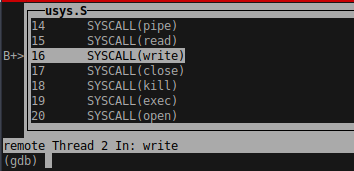
\includegraphics[width=\linewidth-8cm]{layoutsrc.png}
	\end{figure}
	\begin{figure}[H]
		\centering
		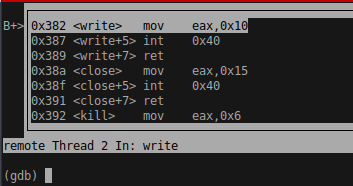
\includegraphics[width=\linewidth-8cm]{layoutasm.png}
	\end{figure}
	
	خروجی دستور 
	\lr{\lstinline|layout src|} 
	خطی از فایل 
	\lr{usys.S} 
	را نشان می‌دهد که منجر به فراخوانی سیستمی 
	\lr{\lstinline|write|} 
	می‌شود.
	
	خروجی دستور 
	\lr{\lstinline|layout asm|} 
	معادل اسمبلی این فرا‌خوانی است. برای فراخوانی سیستمی ابتدا باید شماره‌ی فراخوانی مورد نظر را در ثبات 
	\lr{eax} 
	بریزیم. شماره‌ی فراخوانی‌های سیستمی در سیستم‌ عامل لینوکس در آدرس 
	\lr{/usr/include/x86\_64-linux-gnu/asm/unistd\_64.h} 
	قرار دارند. بعد از این کار باید دستور 
	\lr{\lstinline|syscall|} 
	صدا زده شود که این کار با وقفه‌ی شماره 
	\lr{0x40} 
	صورت گرفته است. در نهایت برای برگشت از تایع کمکی 
	\lr{\lstinline|write|} 
	به فریم تابع 
	\lr{\lstinline|cat|} 
	از دستور 
	\lr{\lstinline|ret|} 
	استفاده شده است.
	قبل از فراخوانی 
	\lr{\lstinline|write|} 
	آرگومان‌های ورودی آن در پشته قرار دارند. این مدل از فراخوانی توابع در سیستم عامل‌های ۳۲ بیتی رواج دارد. در سیستم عامل‌های ۶۴ بیتی چند آرگومان اول نیز همانند شماره‌ی فراخوانی سیستمی در ثبات‌ها قرار ریخته می‌شوند. دستور 
	\lr{\lstinline|ret|} 
	به آدرسی که در سر پشته قرار دارد، برمی‌گردد. این آدرس توسط دستور 
	\lr{\lstinline|call|} 
	در پشته نوشته می‌شود.
\end{itemize}